\chapter{Evaluation}
\label{ch:evaluation}
In this section, we analyze and evaluate the CASC-SAS approach and discuss the findings of the evaluation.
The goal of the evaluation is to derive quantitative and qualitative characteristics of the approach.
These characteristics are used to verify the applicability of the approach in the presented field of application, i.e., the employment of the approach in newly constructed or retrofitted substations.
Furthermore, the characteristics are used to identify limitations and future directions of the approach.

\section{Method}
The evaluation is performed theoretically as well as experimentally.
For the theoretical parts of the evaluation, we employ proofs to demonstrate and guarantee certain characteristics of our approach.
The experimentally performed parts of the evaluation are based on a testbed implementation of our approach and the concepts discussed in \autoref{sec:approach:realization}.
The areas and metrics covered by the different parts of the evaluation are discussed in the following section.

\subsection{Evaluation Areas \& Metrics}
The evaluation of our approach is based on the goal-question-metric (GQM) approach \cite{Basili84,Basili92}.
The GQM approach aims to analyze whether an overall goal was achieved by answering a set of questions that represent the different areas of interest of the evaluation.
These questions are answered by deriving and evaluating quantitative and qualitative metrics.
The evaluation of the CASC-SAS approach covers three areas of interest.
The three areas of interest, i.e., questions to be answered, and their corresponding metrics are defined below:
\begin{description}
    \item[Goal:] Protect the time-constrained and traffic-intensive communication of a newly constructed or retrofitted SAS against domain-typical adversaries and attacks.
    \begin{description}
        \item[Question: Security] Does CASC-SAS provide security against typical SAS adversaries and attacks?
        \begin{description}
            \item[Metric:] Which security, safety, and availability requirements can be satisfied by deploying the approach in a SAS?
            \item[Metric:] Which adversary and system characteristics are assumed?
            \item[Metric:] Which attacks can be mitigated, and how can these attacks be mitigated with regard to their corresponding mitigation strategy?
            \item[Metric:] How does the attack surface of the SAS change?
        \end{description}
        \item[Question: Performance] Is CASC-SAS capable of securing time-constrained and traffic-intensive communication of an SAS in an efficient and scalable manner?
        \begin{description}
            \item[Metric:] Which performance requirements can be satisfied by deploying the approach in a SAS?
            \item[Metric:] Which communication characteristics are assumed?
            \item[Metric:] Which message types are supported?
            % \item Resistance against network exceptions including congestion, delay, jitter, duplicated packets, lost packets, and out-of-order packet delivery
        \end{description}
        \item[Question: Compatibility] Is CASC-SAS a viable solution to enhance the security of newly constructed or retrofitted substations?
        \begin{description}
            \item[Metric:] Which compatibility requirements can be satisfied by deploying the approach in a SAS?
            \item[Metric:] Which device requirements are assumed?
            \item[Metric:] What are the additional costs for SAS construction and retrofitting?
            \item[Metric:] Is the approach feasible with regard to SAS retrofitting?
            % \item Cost-benefit efficiency compared to alternative approaches
        \end{description}
    \end{description}
\end{description}

\subsection{Testbed}
To analyze and evaluate the integration of our approach into the SAS architecture, as discussed in \autoref{sec:approach:realization}, we implemented the approach in hardware and software as a testbed.
The software is implemented component-wise using object-oriented high-level programming languages.
The components are primarily implemented using the programming languages Java and Kotlin.
The software implementation of our approach is published open source on GitHub \cite{gitcasc} under the European Union Public Licence (EUPL) \cite{eupl}.
The implementation is divided into three main packages.
These packages, their sub-packages, and the package interrelationships are shown in \autoref{fig:casc_package_structure}.
The common package contains functionalities that are required by all other parts of the implementation.
Among others, the common package contains classes and interfaces related to message ingress and egress, message serialization, concurrency, and cryptography.
The second package and its sub-packages are dedicated to the CASA components and protocols.
The third package and its sub-packages are dedicated to the SABAAC components and protocols.
To avoid circular dependencies between the packages and achieve loose coupling of components, we employ the dependency inversion principle by using interfaces.
\begin{figure}
    \centering
    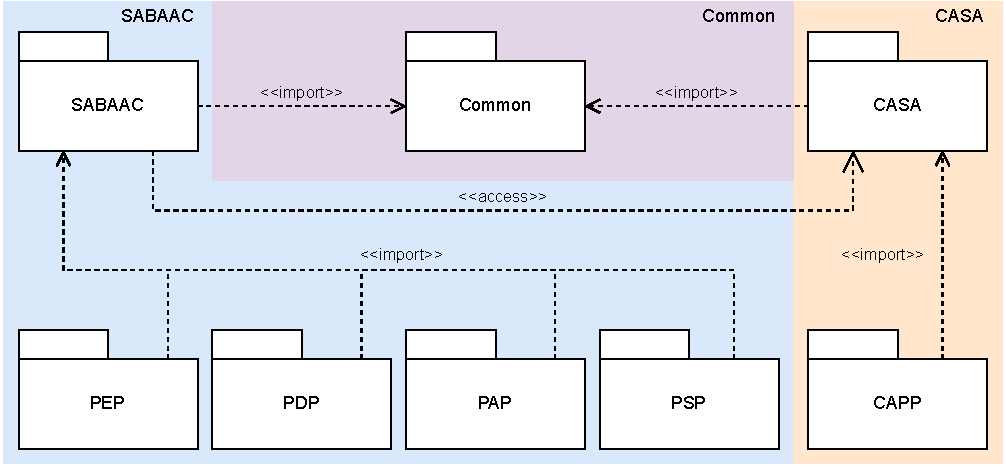
\includegraphics[width=0.9\linewidth]{figures/package_structure.drawio.pdf}
    \caption{Structural package diagram of the CASC-SAS testbed implementation.}
    \label{fig:casc_package_structure}
\end{figure}

To be able to conduct experiments while taking the behavior of physical network communication into account, we transformed the software implementation into a physical system by deploying the SABAAC and CASA components to hardware.
In contrast to deterministic software-based analysis, the testbed evaluation results are practice-oriented and transferable to the SAS domain.
The conceptual topology of our testbed network is visualized in \autoref{fig:evaluation_test_bed}.
The components depicted in blue represent domain-specific devices of an SAS, including IEDs and MUs.
%and computers that mimic the behavior of domain-specific devices of an SAS
The components depicted in yellow represent intermediate network devices for frame and datagram forwarding on the data link layer and network layer.
The components depicted in red are part of the CASC-SAS approach.
The specific hardware used for the experiments is discussed for each experiment individually in the following sections.
\begin{figure}
    \centering
    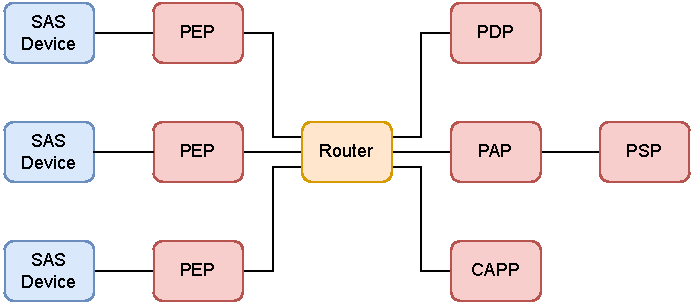
\includegraphics[width=0.8\linewidth]{figures/network_testbed_color.drawio.pdf}
    \caption{Conceptual network topology of the CASC-SAS testbed.}
    \label{fig:evaluation_test_bed}
\end{figure}
%The specific hardware used for the experiments is shown in \autoref{tab:testbed_hardware}.
%We conducted the experiments using a single TTP server that provided the PDP, PAP, PSP, and CAPP services.
%For experiments without real SAS devices, we deployed the PEPs as well as machines that mimic the behavior of domain-specific SAS devices to individual off-the-shelf Raspberry Pi 5 computers.
%For experiments with real IEDs and MUs, only the PEPs were deployed to Raspberry Pi 5 computers.
%
%The simulation and testbed strategy have differing advantages and disadvantages.
%On the one hand, the simulation strategy has the advantage of repeatability and reproducibility due to deterministic behavior, whereas the behavior of the testbed is non-deterministic.

\section{Security Analysis}
In this section, we conduct an analysis of the security of the CASC-SAS approach and its core concepts CASA and SABAAC.
The primary objective of the security analysis is to demonstrate and guarantee certain security-related characteristics of the approach.
As the security analysis is performed theoretically, proofs will be provided demonstrating that the approach is able to mitigate adversarial attacks that endanger these security-related characteristics.
\begin{description}
    \item[Definition.] Unforgeability.\\
    Unforgeability ensures that no adversary can create a valid signature for a message under a policy unless their set of attributes satisfies the policy.
    Unforgeability is defined by using a game between a challenger and an adversary $\mathcal{A}$:
    \begin{itemize}
        \item Setup: The challenger runs the \texttt{Setup} algorithm to generate the public parameters $PK$ and the master secret key $MSK$.
        The public parameters are given to $\mathcal{A}$, while the $MSK$ is kept secret.

        \item KeyGen: $\mathcal{A}$ can query the \texttt{KeyGen} oracle to obtain private keys for sets of attributes of its choice.
        The challenger responds with the corresponding private keys.

        \item SignQueries: $\mathcal{A}$ can request signatures for messages and policies from the \texttt{Sign} oracle.
        The oracle returns valid signatures if the queried attributes satisfy the signing policy.

        \item Forgery: $\mathcal{A}$ outputs a forged signature $(M^*, T^*, \sigma^*)$ for a message $M^*$ and policy $T^*$.
        $\mathcal{A}$ wins if the following conditions hold:
        \begin{itemize}
            \item $\mathcal{A}$ did not request a signature on $(M^*, T^*)$ from the \texttt{Sign} oracle.
            \item $\mathcal{A}$ does not possess a private key whose attributes satisfy the policy $T^*$.
            \item The verification algorithm accepts $\sigma^*$ as a valid signature under $T^*$.
        \end{itemize}
    \end{itemize}

    \item[Definition.] Existential Unforgeability under Chosen-Message Attacks (EU-CMA).\\
    An adversary $\mathcal{A}$ is given access to public parameters, hash oracles, and a signing oracle.
    A scheme is secure if $\mathcal{A}$ cannot forge a valid signature $\sigma^*$ for a new message $M^*$ without knowing the signer's full private key.
    In other words, to create an existential forgery, i.e., create a valid pair of message and signature for a new message, an adversary carrying out a CMA can request valid signatures for any message of his choice \cite{Goldwasser1988}.
    The adversary's advantage in this game is its probability of generating a valid forgery.
    We say the ABS scheme is \textit{existentially unforgeable} if the adversary's advantage is negligible.

    \item[Theorem.] $\mathcal{S}_{CASA}$ is EU-CMA secure under the Computational Diffie-Hellman (CDH) assumption in the random oracle model.\\
    \textit{Proof.} After querying the signing oracle, assume $\mathcal{A}$ forges a signature $\sigma^*$ for $M^*$. The challenger interacts with $\mathcal{A}$ as follows:
    \begin{itemize}
        \item \textit{Setup}: The challenger generates $ppk_i$, $p$, and hash oracles \( H_1, H_2, H_3 \) for \( \mathcal{A} \).
        \item \textit{HashQueries}: The challenger responds to \( H_1, H_2, H_3 \) queries with random values, ensuring consistency.
        \item \textit{SigningQueries}: For $M$ and $\mathsf{Att}_{i}$, the challenger computes:
        \[
        \sigma_i = \big(ppk_{i} \cdot H_3(h)\big)^{\chi_i},
        \]
        where $h = H_2(M || \mathsf{Att}_{i})$.
        \item \textit{Forgery}: If \( \mathcal{A} \) outputs \( \sigma^* \) for \( M^* \), the challenger extracts \( g^{ab} \) from \( g, g^a, g^b \), solving the CDH problem.
    \end{itemize}
    Thus, $\mathcal{A}$'s advantage is negligible under the CDH assumption.
    The $\mathcal{S}_{CASA}$ scheme is secure against EU-CMA attacks.

    \item[Definition.] Collusion Attack.\\
    An adversary $\mathcal{A}$ colludes with a TTP and corrupted signers to derive private keys or forge valid signatures.
    The scheme is secure if such a collusion does not compromise honest signers and does not allow forgery.

    \item[Theorem.] $\mathcal{S}_{CASA}$ resists collusion attacks under the Discrete Logarithm Problem (DLP).\\
    \textit{Proof.} Suppose $\mathcal{A}$ colludes with the CAPP to derive $sk_i = (ppk_i, \chi_i)$, then the following steps are performed:
    \begin{itemize}
        \item The CAPP knows $ppk_i = H_1(\mathsf{ID}_i || \mathsf{ATT}_i)^{s}$.
        \item The signer independently chooses $\chi_i$ and the DLP ensures $\mathcal{A}$ cannot derive $\chi_i$ from $y_i = g^{\chi_i}$.
        \item Without $\chi_i$, $\mathcal{A}$ cannot compute:
        \[
        \sigma_i = \big(ppk_i \cdot H_3(h)\big)^{\chi_i}.
        \]
    \end{itemize}
    Thus, collusion cannot compromise security.
    The $\mathcal{S}_{CASA}$ scheme is secure against collusion attacks.

    \item[Definition.] Message Replay.\\
    To perform a message replay, an adversary captures and repeats the messages exchanged between two or more network devices.
    The adversary aims to inject false data into the system, or disrupt the operation of the network devices.

    \item[Theorem.] CASC-SAS protects SAS devices against message replay attacks.\\
    \textit{Proof.} Suppose two SAS devices, $Alice$ and $Bob$, exchange messages over a network.
    We assume that an adversary $\mathcal{A}$, as introduced in \autoref{sec:approach:attacks}, is able to eavesdrop and replay the messages sent from $Alice$ to $Bob$, and vice versa.
    For the exchange of a message $m$ between $Alice$ and $Bob$, as shown in \autoref{fig:attack_message_replay}, the following steps are performed:
    \begin{itemize}
        \item $Alice$ sends the message $m$ to $Bob$ via $PEP_{Alice}$.
        \item To satisfy the security policies I and IV of CASC-SAS, $PEP_{Alice}$ encapsulates $m$ and a sequence number $seq_m$ in a packet $m' = (Alice, Bob, m, seq_m)$ and signs $m'$ to get $m'' = (m', \sigma_{m'})$.
        \item $PEP_{Alice}$ sends $m''$ to $PEP_{Bob}$ using the network. $PEP_{Bob}$ receives $m''$ from $PEP_{Alice}$, verifies the signature $\sigma_{m'}$, sets the last sequence number received from $PEP_{Alice}$ to $seq_m$, and delivers $m$ to $Bob$.
        \item $\mathcal{A}$ eavesdrops the message exchange, receives $m''$ at the same time as $PEP_{Bob}$, and replays $m''$ to $PEP_{Bob}$.
        \item $PEP_{Bob}$ receives $m''$ from $\mathcal{A}$. As $PEP_{Bob}$ already processed a packet from $PEP_{Alice}$ with sequence number $seq_m$, $m''$ is discarded.
    \end{itemize}
    $\mathcal{A}$ gains no advantage by replaying $m''$, as neither false data is injected into $Alice$ or $Bob$, nor is the operation of $Alice$ or $Bob$ disrupted.
    Thus, SAS devices are protected against message replay attacks.
    \begin{figure}
        \centering
        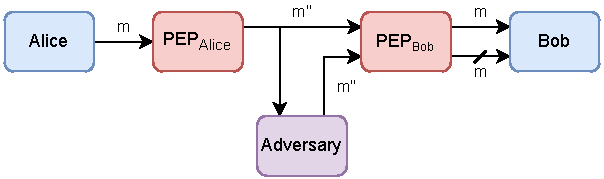
\includegraphics[width=0.75\linewidth]{figures/attack_message_replay.drawio.pdf}
        \caption{Malicious replay of a message exchanged between two PEP-protected SAS devices.}
        \label{fig:attack_message_replay}
    \end{figure}

    \item[Definition.] Message Forgery.\\
    To perform a message forgery, an adversary masquerades as a legitimate device to send malicious messages to other devices.
    By using message forgery, the adversary injects false data into the system, or disrupts the operation of devices.

    \item[Theorem.] CASC-SAS protects SAS devices against message forgery attacks.\\
    \textit{Proof.} Suppose two SAS devices, $Alice$ and $Bob$, exchange messages over a network.
    We assume that only the two devices have the necessary key material to sign and verify exchanged messages.
    As defined in \autoref{sec:approach:attacks}, we assume that an adversary $\mathcal{A}$ is able to initiate arbitrary message exchanges but is unable to bypass or break cryptographic procedures.
    To send a malicious message $m*$ from $\mathcal{A}$ to $Bob$, as shown in \autoref{fig:attack_message_forgery}, $\mathcal{A}$ has to perform the following steps:
    \begin{itemize}
        \item $\mathcal{A}$ creates a message $f$ of its choice.
        \item $\mathcal{A}$ encapsulates $f$ in a packet $m^* = ((Alice, Bob, f, seq_{m^*}), \sigma_{m^*})$, to masquerade as $PEP_{Alice}$.
        \item $\mathcal{A}$ sends $m^*$ to $PEP_{Bob}$.
        \item $PEP_{Bob}$ discards $m^*$ and does not deliver $f$ to $Bob$, as the signature $\sigma_{m^*}$ is not created by $PEP_{Alice}$.
    \end{itemize}
    Since only $PEP_{Alice}$ has the necessary key material to sign messages from $Alice$, $\mathcal{A}$ is unable to masquerade as $Alice$.
    Thus, SAS devices are protected against message forgery attacks.
    \begin{figure}
        \centering
        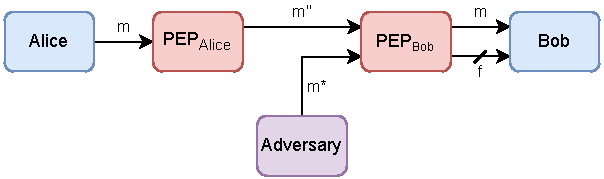
\includegraphics[width=0.75\linewidth]{figures/attack_message_forgery.drawio.pdf}
        \caption{Forgery of a message by masquerading as a PEP-protected SAS device.}
        \label{fig:attack_message_forgery}
    \end{figure}

    \item[Definition.] Message Modification.\\
    To perform a message modification, an adversary captures and alters messages exchanged between two or more network devices.
    Accordingly, message modification is a special type of message forgery that derives a malicious message from a captured message.

    \item[Theorem.] CASC-SAS protects SAS devices against message modification attacks.\\
    \textit{Proof.} Suppose two SAS devices, $Alice$ and $Bob$, exchange messages over a network.
    As with message forgery, we assume that only $Alice$ and $Bob$ have the necessary key material to sign and verify exchanged messages, and that an adversary $\mathcal{A}$ is unable to bypass or break cryptographic procedures.
    We assume that $\mathcal{A}$ performs the attack using a man in the middle approach, i.e., $Alice$ and $Bob$ are not directly connected and the exchanged messages traverse $\mathcal{A}$.
    The modification of a message $m$ from $Alice$ to $Bob$ using a man in the middle approach is shown in \autoref{fig:attack_message_modification}.
    To carry out a message modification attack, $\mathcal{A}$ has to perform the following steps:
    \begin{itemize}
        \item $Alice$ sends the message $m$ to $PEP_{Alice}$.
        \item To satisfy the security policies I and IV of CASC-SAS, $PEP_{Alice}$ encapsulates $m$ and a sequence number $seq_m$ in a packet $m' = (Alice, Bob, m, seq_m)$ and signs $m'$ to get $m'' = (m', \sigma_{m'})$.
        \item $PEP_{Alice}$ sends $m''$ unintentionally to $\mathcal{A}$ using the network.
        \item $\mathcal{A}$ modifies $m$ and encapsulates the modified message $f$ in a packet $m^* = ((Alice, Bob, f, seq_{m}), \sigma_{m})$.
        \item $\mathcal{A}$ sends $m^*$ to $PEP_{Bob}$.
        \item $PEP_{Bob}$ discards $m^*$ and does not deliver $f$ to $Bob$, as the signature $\sigma_{m'}$ does not match the content of $m^*$.
    \end{itemize}
    Since only $PEP_{Alice}$ has the necessary key material to sign messages from $Alice$, $\mathcal{A}$ is unable to renew the signature after modifying the encapsulated message.
    Thus, SAS devices are protected against message modification attacks.
    \begin{figure}
        \centering
        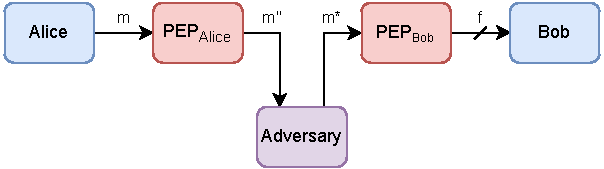
\includegraphics[width=0.75\linewidth]{figures/attack_message_modification.drawio.pdf}
        \caption{Malicious modification of a message exchanged between two PEP-protected SAS devices.}
        \label{fig:attack_message_modification}
    \end{figure}

    \item[Definition.] Time-Delay Attack.\\
    A time-delay attack is the intentional delaying of time-critical messages in a network.
    To perform a time-delay attack, a man in the middle adversary captures a message sent by a network device, and waits a certain time before forwarding it to the message receiver.
    By maliciously delaying exchanged messages, the adversary may either inject outdated data into the system or disrupt the operation of devices.

    \item[Theorem.] CASC-SAS protects SAS devices against time-delay attacks.\\
    \textit{Proof.} Suppose two SAS devices, $Alice$ and $Bob$, exchange messages over a network in the presence of an adversary $\mathcal{A}$, which performs a time-delay attack using a man in the middle approach.
    The performed time-delay attack is shown in \autoref{fig:attack_time_delay}.
    To carry out a message modification attack, $\mathcal{A}$ has to perform the following steps:
    \begin{itemize}
        \item $Alice$ sends the message $m$ to $PEP_{Alice}$.
        \item To satisfy the security policies I and IV of CASC-SAS, $PEP_{Alice}$ encapsulates $m$ with a timestamp-based sequence number $seq_m$ in a packet $m' = (Alice,\allowbreak Bob,\allowbreak m,\allowbreak seq_m)$ and signs $m'$ to get $m'' = (m', \sigma_{m'})$.
        \item $PEP_{Alice}$ sends $m''$ unintentionally to $\mathcal{A}$ using the network.
        \item $\mathcal{A}$ receives $m''$ and waits a certain time before sending it to $PEP_{Bob}$.
        \item $PEP_{Bob}$ discards $m''$ and does not deliver $m$ to $Bob$, as the sequence number $seq_m$ indicates that the packet was maliciously or accidentally delayed.
    \end{itemize}
    The delay of $m''$ would only be unnoticeable if $\mathcal{A}$ was able to update the sequence number.
    However, as only $PEP_{Alice}$ has the necessary key material to sign messages from $Alice$, $\mathcal{A}$ is unable to update the sequence number.
    Thus, SAS devices are protected against time-delay attacks.
    \begin{figure}
        \centering
        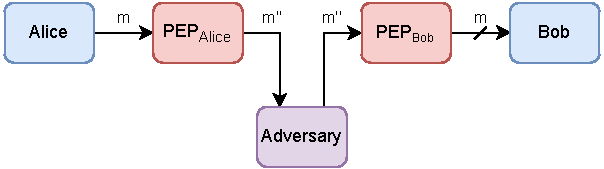
\includegraphics[width=0.75\linewidth]{figures/attack_time_delay.drawio.pdf}
        \caption{Malicious delaying of a message exchanged between two PEP-protected SAS devices.}
        \label{fig:attack_time_delay}
    \end{figure}
    %\item[Theorem.] CASC-SAS protects SAS devices against flooding attacks.\\
    %\textit{Proof.}
\end{description}

\section{Performance Analysis}
In this section, we conduct an analysis of the performance aspects of our approaches CASA and SABAAC.
The objective of the performance analysis is to demonstrate that our approaches are viable solutions to secure message exchanges, taking the strict time and resource constraints of a SAS into account.
For this purpose, we conducted an experimental estimation of message exchange latencies using our testbed implementation and off-the-shelf hardware.
In \autoref{sec:evaluation:performance:setup} the setup of the experiment is discussed in detail.
In \autoref{sec:evaluation:performance:procedure} we describe the procedure and results of the experiment.

\subsection{Experimental Setup}
\label{sec:evaluation:performance:setup}
The testbed of the performance analysis consists of eight devices.
The hardware devices used for the experiment are listed in \autoref{tab:performance_analysis_hardware}.
Two Raspberry Pi 5 were deployed to mimic domain entities that communicate with each other.
Another two Raspberry Pi 5 were used as PEPs protecting the domain entities.
A ThinkPad T480 provided the services of the PAP, PSP, PDP, and CAPP.
\begin{table}
    \centering
    \small
    \caption{Hardware used for the performance analysis testbed.}
    \label{tab:performance_analysis_hardware}
    \begin{tabular}{c c c c}
    \toprule
    Manufacturer & Device & Task & Amount\\
    \midrule
    % SAS Devices
    TP-Link & Omada ER605 & Gigabit Router & 1\\
    % CASA & SABAAC
    Raspberry Pi Ltd & Raspberry Pi 5 8GB & PEP \& Domain Entity & 4\\
    Lenovo & ThinkPad T480 & PDP/PAP/PSP/CAPP & 1\\
    Bechtle & ARTICONA Adapter & USB-A to RJ45 Adapter & 2\\
    \bottomrule
    \end{tabular}
\end{table}

The network topology of the devices used for the performance analysis is shown in \autoref{fig:performance_analysis_topology}.
The PAP, PSP, PDP, CAPP, and PEPs were connected to an industrial grade TP-Link Omada router using Ethernet over twisted-pair.
Each domain entity was connected to its corresponding PEP using Ethernet over twisted-pair, i.e., by using the on-board RJ45 Ethernet connector of the Raspberry Pi 5 domain entity.
However, since the Raspberry Pi 5 only possesses a single on-board RJ45 Ethernet connector, an additional USB-A to RJ45 Ethernet adapter had to be used for both PEPs in order to connect them to the router and to the domain entities.
\begin{figure}
    \centering
    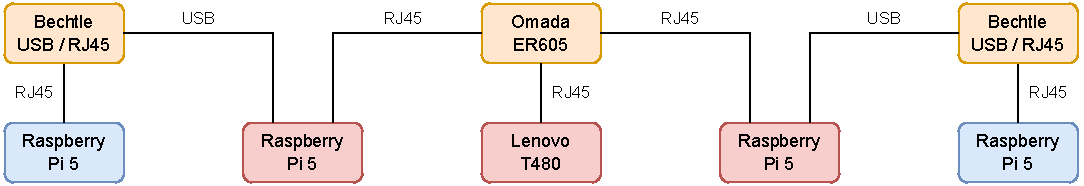
\includegraphics[width=1.0\linewidth]{figures/performance_evaluation_topology.drawio.pdf}
    \caption{Network topology of the performance analysis testbed.}
    \label{fig:performance_analysis_topology}
\end{figure}

\subsection{Procedure \& Results}
\label{sec:evaluation:performance:procedure}
To demonstrate the viability of our approach with regard to securing time critical message exchanges, we aimed to evaluate the extent to which our approach was capable of handling different message types.
For this purpose, we conducted an experiment to estimate the end-to-end communication latency of a message exchange between two domain entities.
The three message types that were considered for the evaluation are discussed in \autoref{sec:approach:system_model:communication:message_types} and listed in \autoref{tab:message_types}.

We realized the message exchange latency estimation by implementing a benchmark program and deploying it to the domain entities.
The benchmark program was implemented in Python.
The program is published open source on GitHub \cite{gitcasc} alongside the implementation of our approach.
The program estimated the end-to-end latency between the two domain entities based on the RTT of a bidirectional message exchange.
We chose UDP as a message exchange protocol for the experiment in order to avoid external latency influences, such as the flow control and congestion control of the Transmission Control Protocol (TCP).
To measure the RTT, the so-called active benchmark entity sent a timestamp to the passive benchmark entity.
The passive entity replied to the message with the received timestamp.
Thus, after receiving the response from the passive entity, the active entity was able to calculate the RTT by subtracting the received timestamp from the current timestamp.
As a consequence, no time synchronization was required between the domain entities.
Furthermore, under the assumption of symmetric transmission times, the accuracy of the RTT measurements only depended on the accuracy of the active entity's system clock.
To avoid RTT fluctuations or an offset caused by the router's buffering and forwarding strategy, messages were sent sequentially, i.e., the active entity waited for the arrival of a response before sending another timestamp message.

The procedure of the experimental latency estimation consisted of ten key events.
The sequence of events and the corresponding messages exchanged between the devices are shown in \autoref{fig:performance_analysis_latency_steps}.
To improve the readability of the shown message exchanges, the USB-A to RJ45 Ethernet adapters were omitted from the figure.
The steps of the experiment procedure are defined in the following:
\begin{description}
    \item[Step 1: Send Request]~\\
    At the initial state of the experiment, no domain-specific messages were exchanged between the devices.
    The necessary key material for signing and verification was already exchanged prior to the experiment.
    The PDP used the precomputed evaluation strategy for access policies, i.e., the access decisions were periodically refreshed and cached.
    The PEPs used a hybrid access decision evaluation strategy, i.e., access decisions were requested and cached as soon as they were needed.
    To initiate the end-to-end latency estimation, the active domain entity sent a UDP packet with its current system clock timestamp to the passive domain entity.

    \item[Step 2: Request Access]~\\
    As the active entity was protected by a PEP, the outgoing UDP packet was captured by the active entity's PEP.
    The PEP checked if an applicable and valid access decision for the packet-related data frames was available in its cache.
    If no applicable or valid access decision was available, the PEP sent an access request to the PDP.

    \item[Step 3: Exchange Request Payload]~\\
    As soon as an applicable and valid access decision was available, the active entity's PEP processed the UDP packet as discussed in \autoref{sec:approach:sabaac:accesscontrol} and sent a payload exchange request to the passive entity's PEP.

    \item[Step 4: Forward Request]~\\
    On receipt of a payload exchange request, the passive entity's PEP verified the request.
    After the request verification, the contained UDP packet was forwarded to the passive domain entity.

    \item[Step 5: Send Response]~\\
    On receipt of the UDP packet, the benchmark program of the passive domain entity extracted the timestamp, created a new UDP packet containing the same timestamp, and sent the new UDP packet to the active domain entity.

    \item[Step 6: Request Access]~\\
    As the passive entity was protected by a PEP, the outgoing UDP packet was captured by the passive entity's PEP.
    The PEP requested and enforced the access decision for the packet as discussed in the second step.

    \item[Step 7: Exchange Response Payload]~\\
    As soon as an applicable and valid access decision was available, the passive entity's PEP processed the UDP response packet and sent a payload exchange request to the active entity's PEP.

    \item[Step 8: Forward Response]~\\
    On receipt of a payload exchange request, the active entity's PEP verified the request and forwarded the contained UDP response packet to the active entity.

    \item[Step 9: Estimate RTT]~\\
    The benchmark program of the active domain entity extracted the timestamp from the response packet and calculated the RTT of the packet by subtracting the received timestamp from the current system clock timestamp.
    To compensate for fluctuations in the RTT measurements and to increase the confidence in the RTT estimation, the active entity repeated the RTT measurement procedure.
\end{description}
\begin{figure}
    \centering
    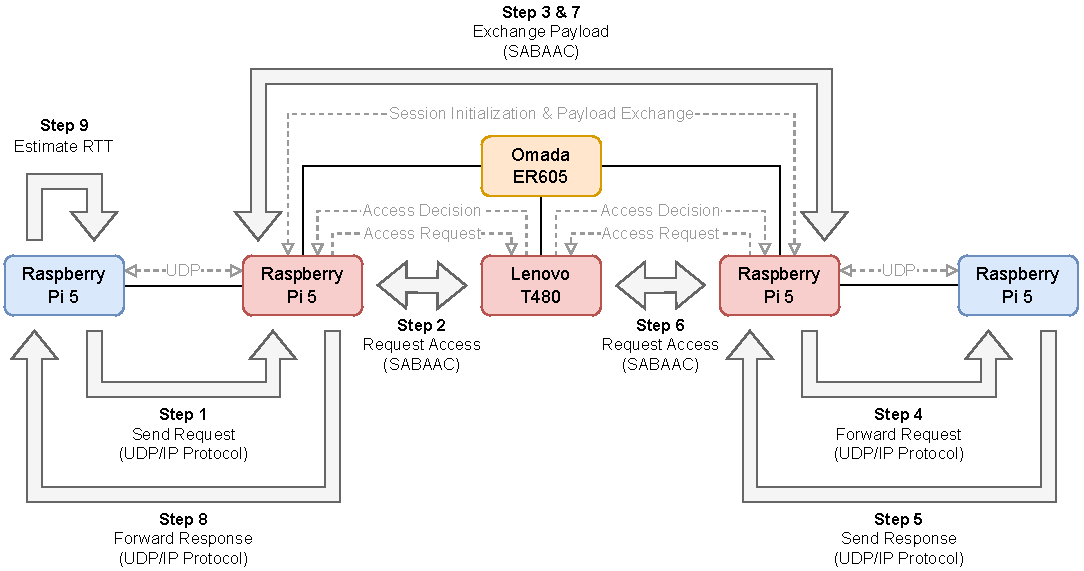
\includegraphics[width=1.0\linewidth]{figures/performance_evaluation_steps.drawio.pdf}
    \caption{Sequence of events of the experimental message exchange latency estimation.}
    \label{fig:performance_analysis_latency_steps}
\end{figure}

The results of the latency estimation experiment are shown in \autoref{tab:rtt_metrics} and \autoref{tab:rtt_share}.
The results are published open source on GitHub \cite{gitcasc} alongside the implementation of our approach.
Since CASA is an algorithm-agnostic approach, we conducted the message exchange latency estimation procedure for six different authentication algorithms.
For each of the authentication algorithms, the benchmark program sent 1000 sequential packets to estimate the RTT.
Based on the measurements, we calculated the arithmetic mean, median, standard deviation, and extrema-related values of each estimation procedure.
Furthermore, we calculated the throughput of the PEPs in Packets Per Second (PPS), and the cumulative share of the 1000 packets in the three message types listed in \autoref{tab:message_types}.

To measure the latency offset caused by packet capturing and forwarding, we performed the initial latency estimation without authorizations, i.e., neither access control nor authentication were used.
From this data, we can see that a bidirectional message exchange between two domain entities requires 1.809 ms on average, which leads to a PEP throughput of 528.2 sequential PPS.
Without authentication, authorization, and access control in place, the measured RTTs are consistent, and each bidirectional message exchange was finished in less than 6 ms RTT, which is required to support the low latency message type.

To measure the influence of the authorization and access control, we performed a latency estimation with authorization and access control but without authentication.
For this purpose, we implemented a so-called no-operation authenticator, which processed the packets without signing or verifying them.
The measurements of the RTTs with the no-operation authenticator show that the authorization and access control workflow of SABAAC leads to an RTT increase of 1.1 ms on average.
Moreover, the increased range of minimum and maximum time indicates that SABAAC leads to an increase in RTT fluctuation.

In order to evaluate the performance of our approach in combination with symmetric cryptography, we performed a latency estimation for HMAC authentication based on SHA-512.
The results show that 99.8 \% of the message exchanges were finished in less than 6 ms RTT.
The remaining two packets or 0.2 \% of the 1000 packets satisfied the 20 ms time constraint of the medium latency message type.
By employing HMAC authentication, CASA and SABAAC achieved a throughput of 289.1 PPS at the PEPs.

To evaluate the performance of our approach in combination with PKC, we conducted latency estimations for three PKC algorithms.
For the latency estimations we chose the Ed25519 algorithm, which is an elliptic-curve digital signature algorithm, RSA-2048, and our $S_{CASA}$ signature scheme.
All three PKC approaches did not satisfy the time constraint of the low latency message type.
Ed25519 and RSA satisfied the time constraint of the medium latency message type.
$S_{CASA}$ was able to finish 99.8 \% of the message exchanges in less than 500 ms, i.e., within the time constraints of the high latency message type.
The data indicates that the RTTs of the PKC approaches are subject to fluctuations with higher magnitude compared to the fluctuations caused by SABAAC and symmetric cryptography.
Furthermore, the throughput of the PEPs was reduced by more than 70 \% compared to the HMAC authentication.
\begin{table}
    \centering
    \small
    \caption{Results of the RTT estimation based on 1000 measurements per authentication algorithm.}
    \label{tab:rtt_metrics}
    \begin{tabular}{c c c c c c c c}
    \toprule
    Authentication & Mean & Median & Deviation & \multicolumn{4}{c}{Extrema}\\
    \cmidrule(lr){5-8}
    & $\bar{x}$ & $\widetilde{x}$ & $\sigma$ & Min & Max & Range & Mid-Range\\
    \midrule
    Unauthorized    & 1.809 & 1.799 & 0.067 & 1.704 & 2.400 & 0.696 & 2.052 \\
    Unauthenticated & 2.937 & 2.924 & 0.146 & 2.808 & 4.213 & 1.405 & 3.511 \\
    HMAC            & 3.342 & 3.279 & 0.507 & 2.779 & 6.695 & 3.915 & 4.736 \\
    Ed25519        & 11.096 & 11.224& 1.591 & 9.537 & 31.971& 22.434 & 20.754 \\
    RSA-2048       & 12.703 & 12.034& 1.179 & 11.741& 16.804& 5.063 & 14.273 \\
    $S_{CASA}$    & 119.851 &113.127&28.534 &111.385&509.392&398.007&310.389\\
    \bottomrule
    \end{tabular}
\end{table}
\begin{table}
    \centering
    \small
    \caption{Throughput and cumulative message type share of the analyzed authentication algorithms.}
    \label{tab:rtt_share}
    \begin{tabular}{c c c c c}
    \toprule
    Authentication & Throughput & \multicolumn{3}{c}{Cumulative Share in Message Types}\\
    \cmidrule(lr){3-5}
     & & Low Latency & Medium Latency & High Latency\\
     & & $\leq 6~ms$ & $\leq 20~ms$ & $\leq 500~ms$\\
    \midrule
    Unauthorized    & 528.2 PPS & 1000 (100 \%) & 1000 (100 \%) & 1000 (100 \%) \\
    Unauthenticated & 328.2 PPS & 1000 (100 \%) & 1000 (100 \%) & 1000 (100 \%) \\
    HMAC            & 289.1 PPS &  998 (99.8 \%)& 1000 (100 \%) & 1000 (100 \%) \\
    Ed25519         &  88.9 PPS &    0 (0 \%)   &  998 (99.8 \%)& 1000 (100 \%) \\
    RSA-2048        &  77.4 PPS &    0 (0 \%)   & 1000 (100 \%) & 1000 (100 \%)\\
    $S_{CASA}$      &   8.2 PPS &    0 (0 \%)   &    0 (0 \%)   &  998 (99.8 \%)\\
    \bottomrule
    \end{tabular}
\end{table}

\section{Compatibility Analysis}
In this section, we conduct an analysis of the compatibility aspects of our approaches CASA and SABAAC.
The objective of the compatibility analysis is to demonstrate that our approach is a viable solution to enhance the communication security in a newly constructed or retrofitted substation.
Accordingly, the compatibility analysis serves the purpose of demonstrating that the SAS behavior and functionality is not influenced by our approach, and that SAS devices protected by CASA and SABAAC are able to provide their services and exchange information.
For this purpose, we conducted a laboratory-based experimental demonstration of applicability with industrial SAS devices.
In \autoref{sec:evaluation:compatibility:setup} the setup of the experiment is discussed.
In \autoref{sec:evaluation:compatibility:procedure} we describe the procedure and results of the experiment.

\subsection{Experimental Setup}
\label{sec:evaluation:compatibility:setup}
In total twelve devices were used to set up the experiment.
The hardware devices used for the experiment are listed in \autoref{tab:lab_hardware}.
Four of these devices were industrial SAS devices, including a MU from General Electric, an IED from ABB, an I/O box from Siemens, and a circuit breaker.
Additionally, a relay test device from Omicron was used to generate three-phase electric power, which was measured by the MU to generate SV frames.
Besides these five SAS-related devices, two Raspberry Pi 5 were used as PEPs.
A ThinkPad T480 provided the services of the PAP, PSP, PDP, and CAPP.
\begin{table}
    \centering
    \small
    \caption{Hardware used for the laboratory-based experimental demonstration of applicability.}
    \label{tab:lab_hardware}
    \begin{tabular}{c c c c c c}
    \toprule
    Manufacturer & Device & Task & SAS & CASC-SAS\\
    \midrule
    % SAS Devices
    General Electric & Reason MU320 & Process Bus Merging Unit & X & \\
    ABB & REL670 & Intelligent Electronic Device & X & \\
    Siemens & SIPROTEC 5 6MD84 & Input/Output Box & X & \\
    Hirschmann & MACH & Managed Ethernet Switch & X & \\
    Hirschmann & RSP35 & Managed Ethernet Switch & X & \\
    OMICRON & CMC 356 & Universal Relay Test Set & X & \\
    / & Circuit Breaker & Electrical Grid Switch & X & \\
    % CASA & SABAAC
    Raspberry Pi Ltd & Raspberry Pi 5 8GB & PEP & & X \\
    Lenovo & ThinkPad T480 & PDP/PAP/PSP/CAPP & & X \\
    Bechtle & ARTICONA Adapter & USB-A to RJ45 Adapter & & X \\
    \bottomrule
    \end{tabular}
\end{table}

The network topology of the devices used for the experiment is shown in \autoref{fig:lab_topology}.
In accordance with the layered SAS architecture shown in \autoref{fig:substation_architecture}, we introduced a layering of devices for the setup of the experiment.
The PAP, PSP, PDP, and CAPP were located at the bay level together with the PEP-protected IED.
As the IED only supported fiber optic network connections, we employed a Hirschmann RSP35 switch as a protocol converter.
With the protocol converter in place, the IED was connected to its PEP using Ethernet over twisted-pair.
The PEP was then connected to a Hirschmann MACH switch representing the process bus switch.
Since the Raspberry Pi 5 only possesses a single on-board RJ45 Ethernet connector, a USB-A to RJ45 Ethernet adapter had to be used for both PEPs.

At the process level of the experiment's network topology the MU was located.
The MU was connected to the relay test device using an analog connection, and was connected to the process bus switch using a fiber optic connection.
Consequently, the MU was not PEP-protected.
In addition to the MU, the PEP-protected I/O box was located at the process level, and was connected to the circuit breaker via an analog connection.
\begin{figure}
    \centering
    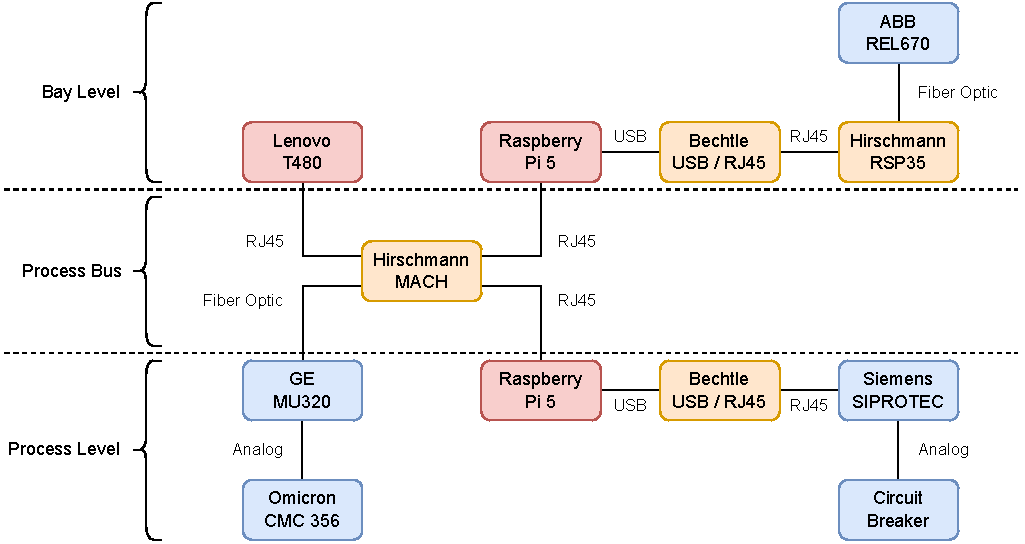
\includegraphics[width=1.0\linewidth]{figures/lab_evaluation_topology.drawio.pdf}
    \caption{Network topology of the laboratory-based experimental demonstration of applicability.}
    \label{fig:lab_topology}
\end{figure}

\subsection{Procedure \& Results}
\label{sec:evaluation:compatibility:procedure}
The procedure of the experiment comprised four key events.
The sequence of events and the corresponding messages exchanged between the devices are shown in \autoref{fig:lab_steps} and are discussed in the following:
\begin{description}
    \item[Step 1: Generate Overcurrent]~\\
    At the initial state of the experiment, the voltages and currents of all three phases generated by the Omicron CMC 356 were within certain boundaries to be detected as normal grid situation.
    Accordingly, the circuit breaker connected to the IED was closed and allowed power to flow through the grid.
    To start the experiment, we manually adjusted the generated three-phase electric power.
    The current was set to a higher level to simulate an overcurrent situation in the grid.
    This situation was communicated to the MU via a direct analog connection, i.e., the MU was measuring the voltages and currents of the three phases.

    \item[Step 2: Send Sampled Values]~\\
    The MU sampled the voltage and current values provided by the relay test device.
    The sampled values were sent to the IED using the SV protocol.
    As the MU was not protected by a PEP, we bypassed the SV frames at the IED's PEP.
    For this purpose, we programmed a static bypass rule into the IED's PEP that analyzed Ethernet frames to detect and forward SV frames sent by the MU.

    \item[Step 3: Send Trip Signal]~\\
    The IED received and processed the SV frames, and detected the overcurrent situation.
    To resolve the overcurrent situation, the IED sent a GOOSE frame to the I/O box to open the circuit breaker.
    As the IED was protected by a PEP, the outgoing GOOSE frame was captured by the PEP and processed as discussed in \autoref{sec:approach:sabaac:accesscontrol}.
    The authenticated and authorized payload exchange message, which contained the GOOSE frame, was then forwarded to the PEP of the I/O box.
    The PEP verified the incoming payload exchange message, extracted the encapsulated GOOSE frame, and forwarded the GOOSE frame to the I/O box.

    \item[Step 4: Trigger Circuit Breaker]~\\
    The I/O box received the original GOOSE frame, which was sent by the IED.
    As the GOOSE frame signalled to the I/O box to open the circuit breaker, the I/O box used an analog signal to open the circuit breaker.
    At the end of the experiment, we were able to visually verify that the circuit breaker had opened successfully.
\end{description}
\begin{figure}
    \centering
    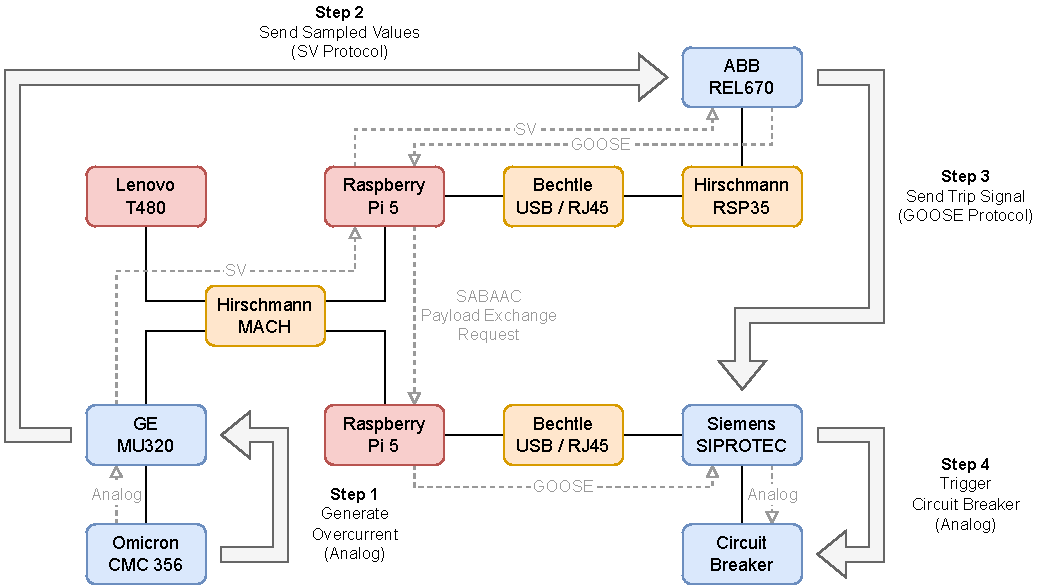
\includegraphics[width=1.0\linewidth]{figures/lab_evaluation_steps.drawio.pdf}
    \caption{Sequence of events of the laboratory-based experimental demonstration of applicability.}
    \label{fig:lab_steps}
\end{figure}

The simulated exception in the grid was successfully propagated through the SAS network during the experiment.
Consequently, the experiment demonstrated that the operation of the MU, IED, and I/O box was not disrupted by the employment of CASA and SABAAC.
Since we deployed the security-related components to inexpensive off-the-shelf hardware, we were able to demonstrate that our approach is a feasible solution for SAS environments not only security-wise and performance-wise but also cost-wise.
Due to the BITW concept of our approach, no adaptations had to be made to the SAS devices.
This indicates that our approach is a viable solution for the retrofitting of existing substations.
Furthermore, the usage of a static bypass rule in one of the PEPs suggests that incompatible or legacy devices could continue their operation in a retrofitted SAS.
Thus, the interoperability and interchangeability requirements of an IEC 61850 substation remain satisfied, while the communication security is increased by the enforcement of the CASC-SAS security policies.

\section{Discussion \& Comparison}
\todo{TODO: Discussion of results and comparison to different approaches}
